\chapter{Sequence Alignment Methods}
\label{ch:alignment}

Before we can understand how genes evolve and how their functions relate across organisms,  we must first learn how to compare biological sequences in a meaningful way.  The comparison of DNA, RNA, and protein sequences lies at the heart of modern bioinformatics, providing the basis for discovering evolutionary relationships, identifying functional regions, and annotating newly sequenced genomes. Sequence alignment is the systematic arrangement of sequences to reveal their similarities and differences. It serves as the foundation for nearly every computational analysis in molecular biology.

\section{Evolution}

In 1973, evolutionary biologist Theodosius Dobzhansky famously declared that ``nothing in biology makes sense except in the light of evolution.''
\marginnote{Dobzhansky T, {\em Am. Biol. Teacher} {\bf 35}, 125–129 (1973)}.
This statement places evolutionary theory at the center of unifying all aspects of biological science. Evolution provides the framework through which the diversity of life, the complexity of organisms, and the relationships among species can be understood. From molecular genetics to ecology, every biological observation gains coherence when viewed as part of an ongoing process of change driven by variation, inheritance, and natural selection. Without evolution, the facts of biology would remain isolated and inexplicable, with it, they form an integrated picture of life’s history and its continuous adaptation to a changing world.

Evolution 
\marginnote{The concept of evolution predates Darwin, with early ideas of species change proposed by naturalists like Jean-Baptiste Lamarck (1809). However, it was Charles Darwin’s {\em On the Origin of Species} (1859) that unified these ideas with a coherent mechanism—natural selection—supported by extensive evidence. Modern evolutionary biology integrates genetics, paleontology, and molecular biology to describe how life has evolved over billions of years.}
is the process by which populations of organisms change over generations through variation (mutations of their genome), inheritance, and selection. Random mutations introduce genetic diversity, while natural selection favors variants that enhance survival or reproduction. Over time, these gradual changes accumulate, producing the diversity of life observed today. "Over time" here is actually an understatement. Evolution had billions of years in order to shape the life as we know it (Table~\ref{t:history-earth}).

\begin{table}[ht]
\centering
\caption{Key events in the history of Earth and life (Ga $=$ billion years ago; Ma $=$ million years ago; ka $=$ thousand years ago).}
\label{t:history-earth}
\begin{tabular}{ll}
\hline
\textbf{Time (approx.)} & \textbf{Event} \\
\hline
4.54 Ga & Formation of Earth \\
4.0--3.8 Ga & Earliest evidence of life (simple microbial activity) \\
3.5 Ga & Emergence of bacteria and prokaryotic cells \\
2.5--2.0 Ga & Rise of atmospheric oxygen \\
2.1--1.8 Ga & Appearance of eukaryotic cells \\
1.2 Ga & Emergence of multicellular organisms \\
700--600 Ma & First animals (sponges and soft-bodied forms) \\
500--475 Ma & First plants colonize land \\
525--500 Ma & Appearance of vertebrates (jawless fish) \\
400--360 Ma & Transition of vertebrates to land (amphibians) \\
200--150 Ma & Evolution of early mammals alongside dinosaurs \\
7--6 Ma & Emergence of hominins (early human ancestors) \\
300--200 ka & Appearance of modern humans (\textit{Homo sapiens}) \\
\hline
\end{tabular}
\end{table}

Historically, evolution was studied by comparing the morphology, that is, the form and structure of organisms. Evolutionary biologists examined fossils, bones, and visible traits of organisms, and compared these to relate them, finding similarities and differences. With advances in molecular biology, scientists began comparing proteins and DNA sequences, enabling much finer resolution. Computational models, statistical inference, and phylogenetic trees now allow the reconstruction of evolutionary relationships from molecular data.

Gene sequences record the history of evolution at the molecular level. Mutations accumulate over time, leaving detectable patterns of similarity and difference among species. By analyzing these patterns computationally, researchers can infer common ancestry, estimate divergence times, and even predict evolutionary pressures.

\section{Homology}

In evolutionary biology 
\marginnote{Evolutionary biology is the branch of biology that studies the origin, change, and diversification of species over time through mechanisms such as mutation, selection, gene flow, and genetic drift.}
and bioinformatics, homologous genes are genes that share a common ancestral origin. They can be classified into two main types: orthologs and paralogs. Orthologous genes arise from a speciation event, meaning they are found in different species but originated from a single gene in the last common ancestor. These genes typically retain the same function across species, making them key for inferring evolutionary relationships and constructing phylogenetic trees. In contrast, paralogous genes result from a gene duplication event within a genome and may evolve new or specialized functions over time. 

Understanding homology—and distinguishing orthologs from paralogs—is crucial in comparative genomics, because it allows researchers to trace gene evolution, predict gene function across species, and reconstruct the molecular history of life.

A classic example of \textbf{orthologs} is the hemoglobin $\beta$-chain gene in humans and the hemoglobin $\beta$-chain gene in whales (or, equivalently, the myoglobin genes in both species). These genes descended from the same ancestral gene in the last common ancestor of humans and whales and retain similar oxygen-binding functions in their respective species, illustrating how mammals adapted to different environments while conserving core physiological mechanisms. Another striking case involves the \textbf{Hox} genes, which control body-plan development in animals: the same basic set of Hox genes that patterns the body of a fruit fly also guides limb and vertebrae formation in humans.

Paralogs, by contrast, showcase how gene duplication propels innovation. Gene duplication is essentially a genetic accident. It occurs when a segment of DNA is copied twice during replication or recombination. While accidental, such duplications provide extra genetic material that evolution can experiment with — one copy maintains the original function, while the other is free to accumulate mutations and potentially evolve new functions. For example, the human globin genes—$\alpha$-globin and $\beta$-globin—originated from a single ancestral gene but duplicated and diverged to specialize in different parts of the hemoglobin molecule, improving oxygen transport. Similarly, the numerous olfactory receptor genes in humans and other mammals arose from repeated duplications, allowing species to detect a wide range of smells.

These examples illustrate how the study of homologous, orthologous, and paralogous genes reveals the deep evolutionary connections among organisms, and how gene duplication and divergence drive the diversity of life’s molecular machinery. They also motivate us to craft algorithmic means of finding these genes, that is, comparing the genetic sequences within the same and between different organisms. The core techniques for sequence comparison are methods that study sequence alignment.

\section{Sequence Alignments}

To understand relationships between genes or proteins, we need a systematic way to compare their sequences. Sequence alignment is the process of arranging two or more DNA, RNA, or protein sequences to identify regions of similarity that may indicate functional, structural, or evolutionary relationships. Alignments reveal where nucleotides or amino acids correspond between sequences, accounting for possible insertions, deletions, or substitutions that occurred over time. 

Beyond evolutionary studies, sequence alignment underlies many tasks in bioinformatics. These include predicting gene or protein function by similarity to known sequences, identifying coding regions in genomes, assembling overlapping fragments in sequencing projects, constructing phylogenetic trees, and searching for orthologs across species. In essence, alignment transforms raw sequence data into biologically meaningful comparisons, providing the foundation for most computational analyses of molecular biology.

Here is an example. Consider two short DNA sequences $s = \texttt{ATACGTA}$ and $t = \texttt{TATGATA}$. The goal of an alignment $A(s,t)$ is to arrange these sequences so that similar characters are aligned in columns, while gaps (denoted by dashes) represent insertions or deletions that occurred during evolution. A possible (perhaps not a very good) alignment is:

\begin{verbatim}
s:  ATACG-TA
        | ||
t:  TAT-GATA
\end{verbatim}

Here, vertical bars indicate matches between the aligned bases. The alignment reveals that the sequences share several conserved positions, while one gap accommodates an insertion or deletion event. Such visual representations help quantify sequence similarity and form the basis for computational algorithms that compare genes or proteins across species.

Here is another alignment of these two sequences:

\begin{verbatim}
s:  ATACG-TA
     || | ||
t:  -TATGATA
\end{verbatim}

Formally, an alignment of sequences $s$ and $t$ can be represented as
$A(s,t) = (x, y)$, where $x$ and $y$ are the aligned versions of $s$ and $t$,
respectively. Each position in $x$ and $y$ contains either a symbol from the
alphabet (e.g., \texttt{A}, \texttt{C}, \texttt{G}, \texttt{T}) or a gap, and
removing the gaps recovers the original sequences.

Which of the above alignments is better? It depends. :)

\section{Alignment Scoring}

To decide which alignment we like best, we need to define an scoring function over the alignment. Let us denote this function as $M(A(s,t))$. The simplest, and surprisingly the most common way to define the scoring, is to break it down to alignment constituents, that is, defined the function over all aligned positions:
\[
M(A(s,t)) = \sum_{i=1}^{L} \sigma(x_i, y_i),
\]
where $L$ is the alignment length, and $\sigma(x_i, y_i)$ is the
\emph{per-symbol scoring function} that assigns a numerical value depending on
whether the aligned characters at position $i$ are a match, mismatch, or gap.

Typical choices for $\sigma(x_i, y_i)$ include positive scores for matches, negative scores for
mismatches, and penalties for gaps. Say,

\[
\sigma(a,b) =
\begin{cases}
-2, & \text{if } a = \texttt{-} \text{ or } b = \texttt{-}, \\
-1, & \text{if } a \neq b \text{ and } a,b \neq \texttt{-}, \\
+2, & \text{if } a = b.
\end{cases}
\]

The optimal alignment is the one that maximizes $M(A(s,t))$ according to the chosen scoring scheme. With two alignments above, and using this scoring function, the alignment score for the first alignment is $-1$, and for the second alignment $+5$ (see Table~\ref{t:step_by_step_scoring}). Of the two alignments, we would prefer the second one.

\begin{table}[h!]
\centering
\caption{Step-by-step scoring of the alignment $A(s,t)$.}
\label{t:step_by_step_scoring}
\begin{tabular}{ccccc}
\hline
\textbf{Position} & \textbf{$x_i$ (s)} & \textbf{$y_i$ (t)} & \textbf{$\sigma(x_i, y_i)$} & \textbf{Explanation} \\
\hline
1 & A & -- & $-2$ & gap in $t$ \\
2 & T & T  & $+2$ & match \\
3 & A & A  & $+2$ & match \\
4 & C & T  & $-1$ & mismatch \\
5 & G & G  & $+2$ & match \\
6 & -- & A & $-2$ & gap in $s$ \\
7 & T & T  & $+2$ & match \\
8 & A & A  & $+2$ & match \\
\hline
\multicolumn{4}{r}{\textbf{Total:}} & $\displaystyle M(A(s,t)) = +5$ \\
\hline
\end{tabular}
\end{table}

\section{Walks Through Alignment Tables}

We can start with thinking of how to systematically search through different alignments. A search table will do. Consider an example, a sequence $s=\texttt{ATGA}$ and a sequence $t=\texttt{TCA}$, and their alignment 

\begin{verbatim}
s: -  A  T  -  G  A
t: T  -  C  A  -  -
\end{verbatim}

We have to admit that this alignment does not look good in terms of score, but it is still a valid one. It can be obtained through a traversal of the alignment table shown in Table~\ref{t:align-table-1}. In this table, we start in the upper-left corner and must finish in the lower-right corner. The allowed moves are to the cell on the right, which corresponds to taking a symbol from one sequence (say, $t$); to the cell below, which corresponds to taking a symbol from the other sequence (say, $s$); or to the cell diagonally down-right, which corresponds to taking symbols from both sequences and aligning them. Notice that moving right or down introduces an insertion or deletion (indel) into one of the sequences.

\begin{table}[h!]
\centering
\caption{A possible traversal of the alignment table for the sequences $s=\texttt{ATGA}$ and $t=\texttt{TCA}$. The numbers indicate the consecutive steps we take in the table, with (0) indicating a start position and (6) a final position in our alignment walk.}
\label{t:align-table-1}
\begin{tabular}{c|cccc}
\hline
 & \texttt{–} & \texttt{T} & \texttt{C} & \texttt{A} \\
\hline
\texttt{–} & (0) & (1) &  &  \\
\texttt{A} &  & (2) &  &  \\
\texttt{T} &  &  & (3) &  (4) \\
\texttt{G} &  &  &  & (5) \\
\texttt{A} &  &  &  &  (6) \\
\hline
\end{tabular}
\end{table}

We can now score the positions of the alignment, and get $-11$ for an alignment score.

\begin{verbatim}
s: -  A  T  -  G  A
t: T  -  C  A  -  -
  -2 -2 -1 -2 -2 -2
\end{verbatim}

Notice that a different alignment results from a different walk in the alignment table. Consider the following alignment with a walk from a Table~\ref{t:align-table-2}:

\begin{verbatim}
s: -  A  T  G  A  -  -  -
t: T  -  -  -  -  -  C  A
\end{verbatim}

\begin{table}[h!]
\centering
\caption{Another possible traversal of the alignment table for the sequences $s=\texttt{ATGA}$ and $t=\texttt{TCA}$.}
\label{t:align-table-2}
\begin{tabular}{c|cccc}
\hline
 & \texttt{–} & \texttt{T} & \texttt{C} & \texttt{A} \\
\hline
\texttt{–} & (0) & (1) &     &  \\
\texttt{A} &     & (2) &     &  \\
\texttt{T} &     & (3) &     &  \\
\texttt{G} &     & (4) &     &  \\
\texttt{A} &     & (5) & (6) & (7) \\
\hline
\end{tabular}
\end{table}

The scoring of the positions in this alignment is shown below, with the final total score of $-14$, which is even worse than that of our previous alignment:

\begin{verbatim}
s: -  A  T  G  A  -  -  -
t: T  -  -  -  -  -  C  A
  -2 -2 -2 -2 -2 -2 -2 -2
\end{verbatim}

However, notice something important: the two alignments share the same initial part of the walk. Up to position (2), both walks are identical, and therefore the score up to that point (which is $-4$) is the same as well. Once we have computed the score for a particular portion of the walk, there is no need to recompute it if another alignment shares that portion:

\begin{verbatim}
s: -  A | T  -  G  A
t: T  - | C  A  -  -

s: -  A | T  G  A  -  -  -
t: T  - | -  -  -  -  C  A
\end{verbatim}

The total score of the alignment up to the position marked with {\tt |} is $-4$ for both walks. The realization that shared parts of the walk need to be computed only once leads to a very  efficient alignment scoring algorithm—and, ultimately, to an algorithm that can find the  highest-scoring alignment.

\section{A Search for the Best Alignment}

Given two biological sequences, our goal is to find the alignment that achieves the highest possible score according to a chosen scoring scheme. In principle, one could generate \emph{all} possible alignments of the two sequences, compute their scores, and select the best one. However, this exhaustive approach quickly becomes infeasible even for short sequences. For instance, when each sequence has only ten symbols, there are already on the order of $1.9\times 10^5$ possible alignments, and for sequences of length twenty, this number explodes to more than $10^{11}$. A more efficient method is required.

Formally, let $\mathcal{A}(s,t)$ denote the set of all possible alignments between sequences $s$ and $t$. 
For any alignment $A \in \mathcal{A}(s,t)$, let $M(A)$ represent its alignment score. 
The \emph{optimal alignment}, denoted by $A^*(s,t)$, is the alignment that maximizes the scoring function:
\[
A^*(s,t) = \arg\max_{A \in \mathcal{A}(s,t)} M(A),
\qquad
M(A^*) = \max_{A \in \mathcal{A}(s,t)} M(A),
\]
%
so that for all possible alignments $A$,
%
\[
M(A^*) \ge M(A).
\]

A key observation, stemming from our alignment walks above, is that an optimal alignment of two sequences can be built \emph{incrementally}. Suppose we have already computed the best possible alignment for the prefixes of the two sequences up to certain positions. When we extend these prefixes by one additional symbol (or introduce a gap), the best alignment for the longer prefixes can be obtained directly from these previously computed partial results. In other words, the problem exhibits an \emph{optimal substructure}: the optimal solution to the whole problem can be constructed from the optimal solutions to its smaller subproblems.

This insight leads naturally to the \textbf{Needleman–Wunsch algorithm}, 
\marginnote{The Needleman–Wunsch algorithm was introduced by Saul B. Needleman and Christian D. Wunsch in 1970 ({\em Journal of Molecular Biology}) and was the first dynamic programming method for global sequence alignment. It guarantees finding the optimal alignment between two sequences according to a defined scoring scheme and laid the foundation for modern bioinformatics.}
a dynamic programming method that systematically computes the best possible alignment score by filling in a matrix of partial results. We refer to this matrix as the \textbf{dynamic programming table}. Each cell of the table, denoted by $M_{ij}$, represents the best possible alignment score between the prefixes $s_1 s_2 \ldots s_i$ of the first sequence and $t_1 t_2 \ldots t_j$ of the second sequence.

The value of $M_{ij}$ is computed recursively from the neighboring cells, based on whether the last step in the alignment was a match/mismatch, a gap in $s$, or a gap in $t$:

\[
M_{ij} = \max
\begin{cases}
M_{i-1,\,j-1} + \sigma(s_i, t_j), & \text{(align $s_i$ with $t_j$)}\\[6pt]
M_{i-1,\,j} + \sigma(s_i, \texttt{-}), & \text{(gap in $t$)}\\[6pt]
M_{i,\,j-1} + \sigma(\texttt{-}, t_j), & \text{(gap in $s$)}.
\end{cases}
\]

The first row and column of the matrix are initialized with cumulative gap penalties, and the final cell $M_{mn}$ (where $m$ and $n$ are the lengths of the sequences) gives the score of the optimal global alignment. It also helps us if we remember which of the three moves is the one we took to get the maximum value at each particular cell. 


\begin{table}[h!]
\centering
\caption{Dynamic programming table with scores $M_{ij}$ for $s=\texttt{ATGA}$ and $t=\texttt{TCA}$.}
\label{t:dpt}
\begin{tabular}{c|cccc}
\hline
 & \texttt{–} & \texttt{T} & \texttt{C} & \texttt{A} \\
\hline
\texttt{–} & \textbf{0}  & -2 & -4 & -6 \\
\texttt{A} & \textbf{-2} & -1 & -3 & -1 \\
\texttt{T} & -4 & \textbf{0} & -2 & -2 \\
\texttt{G} & -6 & -2 & \textbf{-1} & -3 \\
\texttt{A} & -8 & -4 & -3 & \textbf{-1} \\
\hline
\end{tabular}
\end{table}

Consider the dynamic programming table for the alignment of our two sequences (Table~\ref{t:dpt}). The numbers marked in bold indicate a path we take for optimal alignment. Based on the optimal walk through this table, we find that the optimal alignment is
\begin{verbatim}
s: A  T  G  A
      |  |  |
t: -  T  C  A
\end{verbatim}
and its score is $+1$.

It is important to note that, in some cases, more than one move may yield the same optimal value for a given cell in the dynamic programming table. Such \emph{ties} indicate that multiple paths can lead to the same overall alignment score. Consequently, there may exist several distinct alignments that all achieve the optimal score. In practice, one of these paths can be chosen arbitrarily when tracing back through the table, since all represent equally optimal solutions under the given scoring scheme.

\section{A Note on Dynamic Programming}

Dynamic programming, a term coined by Richard Bellman in the 1950s,
\marginnote{\raggedright Bellman, R. (1952). On the Theory of Dynamic Programming. {\em Proc. of the National Academy of Sciences of the USA}, 38(8), 716–719.} is named to describe a method of solving complex problems by breaking them down into simpler subproblems. Bellman chose the term "dynamic programming" for strategic reasons. At the time, he was working with the U.S. government, where the word "programming" was a popular term and had positive associations, particularly in operations research and planning. By adding "dynamic," he aimed to emphasize the method's focus on time-evolving processes, as the problems it addressed often involved sequences of decisions over time.

In dynamic programming, 
\marginnote{Needleman and Wunsch were aware of Richard Bellman’s work on dynamic programming and based their method directly on his principle of optimality. They were the first to apply dynamic programming to biological sequence alignment, which made their 1970 paper so influential.}
solutions to subproblems are stored (or "memorized") to avoid redundant calculations, which makes it particularly efficient for problems with overlapping subproblems, like shortest path, sequence alignment, and optimization problems. The approach dynamically combines solutions to smaller subproblems to build up the solution to the original, larger problem, leading to a highly structured and systematic way of tackling complex problems.

\section{Local Alignment}

While the Needleman--Wunsch algorithm 
\marginnote{Smith and Waterman built directly on the Needleman–Wunsch algorithm. In their 1981 paper ({\em J. Mol. Biol.}), they added a simple zero term to the recurrence, converting global alignment into local alignment and enabling detection of high-scoring subsequence matches.}
searches for the best \emph{global} alignment between two complete sequences, many biological problems require identifying regions of local similarity instead. For example, two proteins may share only one conserved domain or motif, while the rest of their sequences differ substantially. The goal of \textbf{local alignment} is therefore to find the pair of subsequences that produce the highest alignment score, rather than aligning the sequences end to end. This approach was formalized by \textbf{Smith and Waterman} in 1981, who modified the dynamic programming formulation to reset negative scores to zero, ensuring that only high-scoring local regions are extended. Local alignment is particularly useful for database searches and for detecting conserved functional regions within otherwise unrelated sequences.

The recurrence relation for the local alignment score is defined as:

\[
M_{ij} = \max
\begin{cases}
0, & \text{(start a new alignment)}\\[6pt]
M_{i-1,\,j-1} + \sigma(s_i, t_j), & \text{(match or mismatch)}\\[6pt]
M_{i-1,\,j} + \sigma(s_i, \texttt{-}), & \text{(gap in $t$)}\\[6pt]
M_{i,\,j-1} + \sigma(\texttt{-}, t_j), & \text{(gap in $s$)}.
\end{cases}
\]

By including the zero term, the algorithm discards regions with negative cumulative scores
and effectively identifies the highest-scoring subsequence pair. The maximum value in the
matrix corresponds to the optimal local alignment score, and a traceback starting from that
cell reveals the aligned region.



Here is an example. Consider two sequences, $s =$ \texttt{ACCTGAA} and $t =$ \texttt{CGTGACG}, and the scoring function:
\[
\sigma(a,b) =
\begin{cases}
+2, & \text{if } a = b,\\[4pt]
-1, & \text{if } a \neq b,\\[4pt]
-2, & \text{if } a = \texttt{-} \text{ or } b = \texttt{-}.
\end{cases}
\]

Applying the Smith--Waterman algorithm gives the dynamic programming table shown in Table~\ref{t:smith-waterman}. 
The maximum value in the table (\textbf{8}) corresponds to the best local alignment between the two sequences.

\begin{table}[h!]
\centering
\caption{Dynamic programming table for local alignment of $s=\texttt{ACCTGAA}$ and $t=\texttt{CGTGACG}$. 
The bold numbers indicate the cells on an optimal local-alignment path.}
\label{t:smith-waterman}
\begin{tabular}{c|cccccccc}
\hline
 & \texttt{–} & \texttt{C} & \texttt{G} & \texttt{T} & \texttt{G} & \texttt{A} & \texttt{C} & \texttt{G} \\
\hline
\texttt{–} & 0 & 0 & 0 & 0 & 0 & 0 & 0 & 0 \\
\texttt{A} & 0 & 0 & 0 & 0 & 0 & 2 & 0 & 0 \\
\texttt{C} & 0 & \textbf{2} & 0 & 0 & 0 & 0 & 4 & 2 \\
\texttt{C} & 0 & 2 & \textbf{1} & 0 & 0 & 0 & 2 & 3 \\
\texttt{T} & 0 & 0 & 1 & \textbf{3} & 1 & 0 & 0 & 1 \\
\texttt{G} & 0 & 0 & 2 & 1 & \textbf{5} & 3 & 1 & 2 \\
\texttt{A} & 0 & 0 & 0 & 1 & 3 & \textbf{7} & 5 & 3 \\
\texttt{A} & 0 & 0 & 0 & 0 & 1 & 5 & 6 & 4 \\
\hline
\end{tabular}
\end{table}

The highest-scoring cell (in bold) has a value of $7$, marking the end of the best local alignment. 
Tracing back from that cell reveals the following aligned subsequences:

\begin{verbatim}
s: A C C T G A A
     |   | | |
t:   C G T G A C G
\end{verbatim}

Thus, the Smith--Waterman algorithm identifies the local region \texttt{CCTGA} in $s$ and \texttt{CGTGA} in $t$ as the best-matching subsequences, with an optimal local alignment score of $7$.


\section{An Example: Longest Common Subsequence}

Let us now diverge a bit, and instead of alignments use dynamic programming for a similar problem of finding the longest common subsequence. The \textbf{longest common subsequence (LCS)} of two sequences is the longest sequence that appears in both of them in the same order, but not necessarily contiguously. For example, for $s=\texttt{ACDBE}$ and $t=\texttt{ABCDE}$, the longest common subsequence is $\texttt{ACDE}$, which has length four. The LCS problem captures the idea of sequence similarity without considering insertions, deletions, or substitutions explicitly, and serves as a simplified model for understanding alignment algorithms.

We first need to define the scoring mechanism for traversal of the dynamic programming table. We do not gain in the length of the longest common subsequence if we take only a symbol from one of the sequences, but we gain a length of $1$ if we take symbols from both sequences and they are equal. This can be expressed using a simple scoring function
\[
\sigma(a,b) =
\begin{cases}
1, & \text{if } a = b,\\[4pt]
0, & \text{if } a \neq b.
\end{cases}
\]
The recurrence relation for computing the entries of the dynamic programming table is then
\[
M_{ij} = \max
\begin{cases}
M_{i-1,\,j-1} + \sigma(s_i, t_j), & \text{(take both symbols)}\\[6pt]
M_{i-1,\,j}, & \text{(skip a symbol from $s$)}\\[6pt]
M_{i,\,j-1}, & \text{(skip a symbol from $t$)}.
\end{cases}
\]

Now to the code. We first define the scoring function:

\vspace*{3mm}
\begin{lstlisting}
def score(a, b):
    return 1 if a == b else 0
\end{lstlisting}

This was easy. Now, the main algorithm, the construction of the dynamic programming table. We use a trick: besides computing the scores we will also remember the neighboring cells (up and to the left) from which these scores originated. This will allow us to trace back for the solution of the problem:

\vspace*{3mm}
\begin{lstlisting}
def longest_common_subsequence(s, t):
    M = defaultdict(int)
    P = {}
    for i, si in enumerate(s):
        for j, tj in enumerate(t):
            M[i, j], P[i, j] = max(
                (M[i-1, j], (i-1, j)),
                (M[i, j-1], (i, j-1)),
                (M[i-1, j-1] + score(si, tj), (i-1, j-1))
            )
    return M, P
\end{lstlisting}

After filling in the dynamic programming table $M$, we must recover the actual longest common subsequence by retracing the path of decisions that led to the optimal score. We do this by following the pointers stored in $P$, which indicate which previous cell contributed to the current maximum:

\vspace*{3mm}
\begin{lstlisting}
def trace_back(s, t, M, P):
    i = len(s)-1
    j = len(t)-1
    result = ""
    while M[i, j] != 0:
        if P[i, j] == (i - 1, j - 1):
            result = s[i] + result
        i, j = P[i, j]
    return result
\end{lstlisting}

Finally, we can run the algorithm on two example sequences and display the result:

\vspace*{3mm}
\begin{lstlisting}
s = "AACCTTGG"
t = "ACACTGTGA"
table, previous = longest_common_subsequence(s, t)
substring = trace_back(s, t, table, previous)
print(f"Longest common subsequence: {substring}")
print(f"Length: {table[len(s) - 1, len(t) - 1]}")

\end{lstlisting}

The program outputs:

\vspace*{3mm}
\begin{lstlisting}
Longest common subsequence: AACTTG
Length: 6
\end{lstlisting}

It works! This example demonstrates how dynamic programming can efficiently recover not only the score but also the actual subsequence representing the shared structure between two sequences. The reader can now extend the code to output the actual dynamic programming table, show its entries and highlight the optimal path.

\section{Alignment with Affine Gap Penalties}

So far, we have assumed that each gap in an alignment incurs a linear penalty proportional to its length. 
However, in biological sequences, it is often more realistic to distinguish between the cost of \emph{opening} a gap 
and the cost of \emph{extending} it. Introducing a new gap typically reflects a separate mutational event and 
should therefore be penalized more heavily than simply extending an existing one. 

To capture this, we define an \textbf{affine gap penalty function}:
\[
\gamma(g) = -(\rho + \varepsilon \times x),
\]
where $\rho$ is the cost of \emph{opening} a gap, $\varepsilon$ is the cost of \emph{extending} a gap by one symbol, 
and $x$ is the length of the gap. For example, if $\rho = 5$ and $\varepsilon = 1$, then a gap of length three 
would have a penalty of $-(5 + 3\times1) = -8$. This scheme penalizes multiple short gaps more severely than 
a single long one, which better reflects biological reality.

A simple dynamic programming table, as used in the Needleman–Wunsch algorithm, is insufficient for affine gap penalties. 
That approach assumes that each cell depends only on the immediately adjacent cells (diagonal, above, and left). 
With affine gaps, however, we must distinguish between whether we are \emph{continuing} a gap or 
\emph{starting} a new one. This requires keeping track of the direction from which we arrived at each cell.

To handle this, we maintain three separate dynamic programming matrices:
\[
\begin{cases}
M_{ij}^\downarrow & \text{(gap in $t$ — moving down)},\\[4pt]
M_{ij} & \text{(match or mismatch — moving diagonally)},\\[4pt]
M_{ij}^\rightarrow & \text{(gap in $s$ — moving right)}.
\end{cases}
\]

Each of these matrices represents the best possible score of an alignment ending at position $(i,j)$ 
under the given condition. Their recurrences are defined as follows:

\[
M_{ij}^\downarrow = \max
\begin{cases}
M_{i-1,\,j}^\downarrow - \varepsilon, & \text{(extend a gap in $t$)}\\[4pt]
M_{i-1,\,j} - \rho, & \text{(open a new gap in $t$)}
\end{cases}
\]

\[
M_{ij}^\rightarrow = \max
\begin{cases}
M_{i,\,j-1}^\rightarrow - \varepsilon, & \text{(extend a gap in $s$)}\\[4pt]
M_{i,\,j-1} - \rho, & \text{(open a new gap in $s$)}
\end{cases}
\]

\[
M_{ij} = \max
\begin{cases}
M_{i-1,\,j-1} + \sigma(s_i, t_j), & \text{(match or mismatch)}\\[4pt]
M_{ij}^\downarrow, & \text{(from a gap in $t$)}\\[4pt]
M_{ij}^\rightarrow, & \text{(from a gap in $s$)}.
\end{cases}
\]

Together, these three matrices correctly account for affine gap penalties, 
allowing the algorithm to distinguish between opening and extending gaps 
while still guaranteeing an optimal alignment through dynamic programming.

The traversal for finding the best alignment score now involves moving \emph{across all three matrices} rather than within a single one. At each position $(i,j)$, the algorithm considers transitions not only from neighboring cells within the same matrix but also from corresponding cells in the other two matrices. The optimal path, therefore, may switch between $M_{ij}$, $M_{ij}^\downarrow$, and $M_{ij}^\rightarrow$, depending on whether the alignment continues a match, opens a new gap, or extends an existing one.  The traceback procedure follows this combined path across the three matrices, starting from the cell with the highest overall score and reconstructing the optimal alignment by identifying, step by step, which operation (match, gap opening, or gap extension) was taken. This traversal is illustrated schematically in Figure~\ref{f:affine-gap-traversal}.

\begin{figure}[ht]
    \centering
    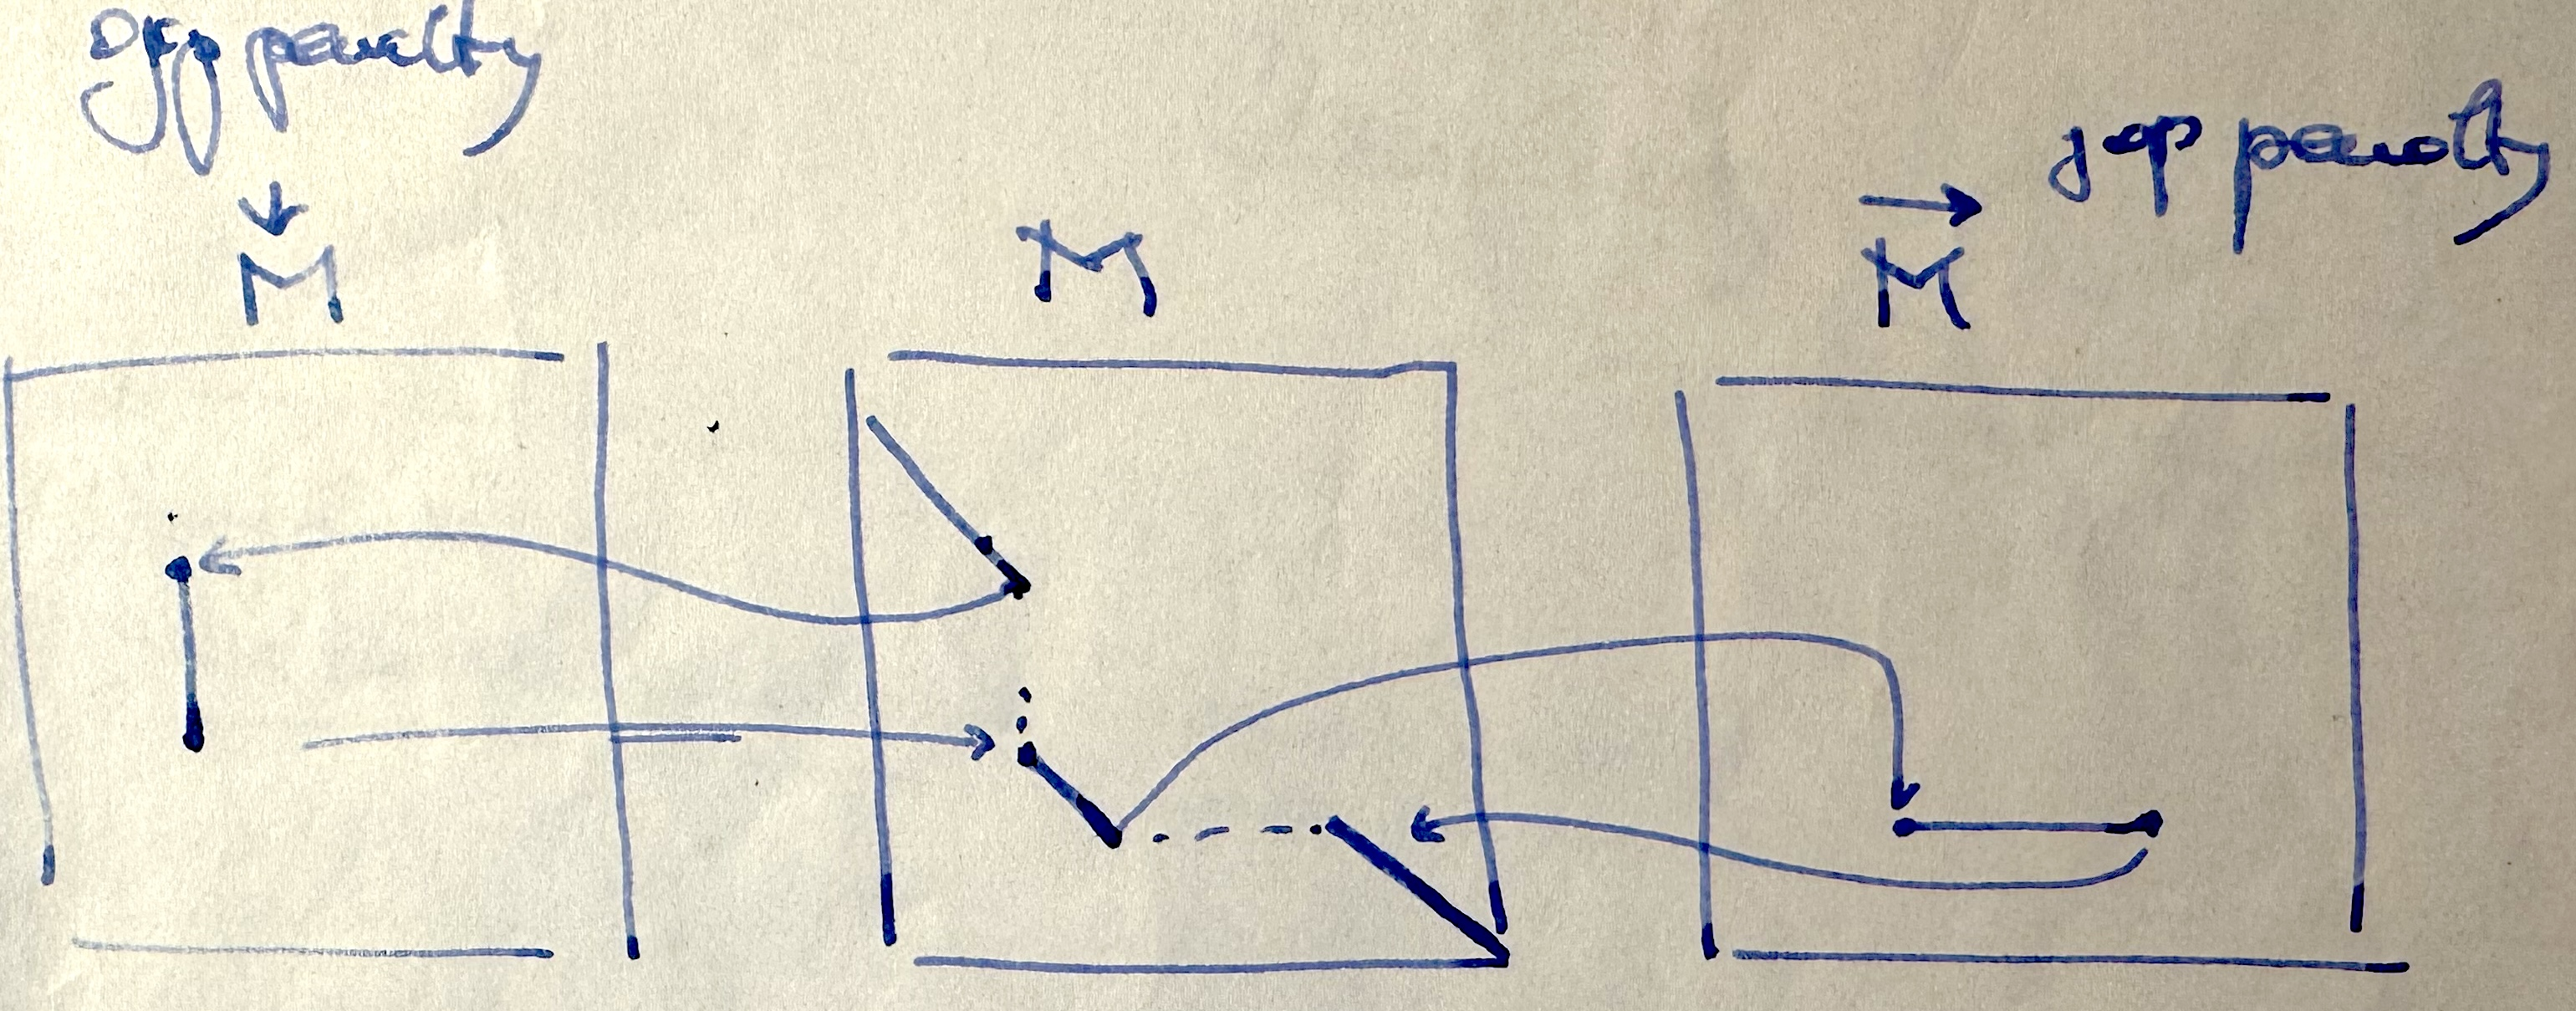
\includegraphics[width=0.99\textwidth]{figs/alignment/affine.jpg}
    \caption{An example of traversal of the three dynamic programming tables for the alignment with affine gap penalties.}
    \label{f:affine-gap-traversal}
\end{figure}

\section{Multiple Sequence Alignment}

Pairwise alignment methods, such as the Needleman–Wunsch and Smith–Waterman algorithms, form the basis of comparing two sequences optimally. However, many biological analyses require comparing whole families of sequences simultaneously. Extending these ideas to three or more sequences leads to the problem of multiple sequence alignment, which generalizes pairwise alignment but introduces new computational challenges. Such comparisons may consider different versions of a gene across species or members of a protein family within the same organism. To reveal regions that have remained similar over time and to understand how the sequences relate evolutionarily, we align all of them together in what is called a multiple sequence alignment. 

A multiple sequence alignment arranges three or more sequences in a table so that symbols with a shared evolutionary origin appear in the same column. For example:
%
\begin{verbatim}
s1: A T - G C A
s2: A T G G - A
s3: A T T G C A
\end{verbatim}
%
This alignment highlights conserved positions (“A–T–G–A”) and regions that have changed through mutations, insertions, or deletions. 

The Needleman--Wunsch algorithm can, in principle, be extended to align more than two sequences. Instead of filling a two-dimensional dynamic programming table, we would construct a table with one dimension for each sequence, where each cell represents the best alignment score for the corresponding prefixes of all sequences. For three sequences, this becomes a three-dimensional cube; for four, a four-dimensional hypercube, and so on. Each additional sequence therefore adds another dimension to the computation. The number of possible paths through this multidimensional table grows exponentially, requiring both time and memory on the order of $O(n^k)$, where $n$ is the sequence length and $k$ is the number of sequences. While this exact dynamic programming approach guarantees an optimal multiple sequence alignment, it quickly becomes impractical. As a result, nearly all practical methods rely on heuristics or approximations that trade exact optimality for tractable computation.

Because exact multiple sequence alignment by dynamic programming is computationally infeasible for more than a few short sequences, practical methods rely on heuristics that approximate the optimal result. One of the most common strategies is progressive alignment. Instead of aligning all sequences at once, the algorithm builds the alignment step by step. First, all pairs of sequences are aligned to estimate their similarities, which are then used to construct a guide tree 
\marginnote{The construction of the guide tree relies on pairwise sequence similarities and forms the basis for clustering algorithms such as \textit{neighbor joining}, which can infer phylogenetic relationships among sequences. We will explore these methods in a later chapter.}
representing their approximate relationships. The two most similar sequences are aligned first, and the resulting alignment is treated as a single entity called a profile.  

A profile summarizes each column of the current alignment by recording how often each nucleotide or amino acid appears there. When a new sequence is added, it is aligned against this profile rather than against individual sequences, choosing the placement that best matches the column frequencies. The process continues until all sequences have been incorporated.  

For example, given three DNA sequences  
\[
\texttt{s}_1 = \texttt{ATGA}, \quad 
\texttt{s}_2 = \texttt{ATGCA}, \quad 
\texttt{s}_3 = \texttt{ATGGA},
\]
the algorithm might first align $\texttt{s}_1$ and $\texttt{s}_2$:
\begin{verbatim}
s1: A T G - A
s2: A T G C A
\end{verbatim}
The resulting profile represents each column as a distribution of residues (for instance, the fourth column has 50\% gaps and 50\% C). The third sequence, $\texttt{s}_3$, is then aligned against this profile to produce the final multiple alignment.

The quality of such an alignment is often measured by the \textbf{sum-of-pairs score}, which adds the scores of all pairwise comparisons implied by the alignment. Columns with matching or chemically similar residues contribute positively, while mismatches and gaps reduce the total.  

An alternative, information-based measure uses \textbf{entropy} to quantify conservation within each column:
\[
H = -\sum_{i=1}^{k} p_i \log_2 p_i,
\]
where $p_i$ is the frequency of residue $i$ and $k$ is the alphabet size. A completely conserved column, where all sequences have the same residue, has $H = 0$; a highly variable one has higher entropy. For example, if 8 out of 10 residues in a column are A and 2 are G, then $H \approx 0.72$.  

Low-entropy columns signal conserved, biologically important regions, while high-entropy columns mark variable positions. Together, these scoring schemes provide complementary ways to evaluate the quality of a multiple sequence alignment, balancing sequence similarity with biological relevance.

Multiple sequence alignments provide the foundation for many downstream analyses in bioinformatics. They are used to identify conserved motifs that indicate important structural or functional sites, to build phylogenetic trees that reconstruct evolutionary relationships, and to generate profiles or hidden Markov models for sequence classification. High-quality alignments are thus critical inputs for comparative genomics, structural prediction, and protein family analysis.

\section{A Note on Scoring Functions for Nucleotide Alignment}

When aligning nucleotide sequences, the scoring function determines the numerical reward or penalty assigned to each possible pairing of nucleotides or gaps. The choice of scoring system has a strong influence on the resulting alignment, especially when gaps are present or when substitution biases exist in the data.

The scoring function we have used above (match = +2, mismatch = -1, gap = -2) is a simple symmetric scheme that treats all nucleotide substitutions equally and applies a uniform penalty for gaps. It assumes that all substitutions and all gaps are equally costly.  While it may is sufficient for illustrating the mechanics of global or local alignment algorithms such as Needleman–Wunsch or Smith–Waterman, in biological data, however, substitutions between nucleotides are not all equally likely.  For instance, in DNA or RNA, the four bases (A, C, G, and T or U) exhibit a strong transition/transversion bias:

\begin{itemize}
    \item Transitions (A$\leftrightarrow$G and C$\leftrightarrow$T) occur more frequently,
    \item Transversions (A$\leftrightarrow$C, A$\leftrightarrow$T, G$\leftrightarrow$C, G$\leftrightarrow$T) occur less frequently.
\end{itemize}

To reflect this bias, one can design a substitution matrix in which transitions are penalized less heavily than transversions. In scoring Table~\ref{tab:nt_substitution_matrix}, transitions (A$\leftrightarrow$G, C$\leftrightarrow$T) receive a penalty of $-0.5$, while transversions are penalized by $-1.5$.

\begin{table}[htbp]
\caption{Example of a nucleotide substitution matrix reflecting transition bias.}
\label{tab:nt_substitution_matrix}
\centering
\begin{tabular}{c|rrrr}
  & A & C & G & T \\
  \hline
  A & +1 & -1.5 & -0.5 & -1.5 \\
  C & -1.5 & +1 & -1.5 & -0.5 \\
  G & -0.5 & -1.5 & +1 & -1.5 \\
  T & -1.5 & -0.5 & -1.5 & +1 \\
\end{tabular}
\end{table}

More sophisticated scoring functions can be derived empirically.
\marginnote{An alternative is to use explicit substitution models such as Kimura models that describe the evolutionary processes with parameters like the transition/transversion ratio and base frequencies. More on such models in later chapters.}
For instance, from a large collection of trusted alignments, say, from a library of homologous sequences, one can estimate the joint probability $P(a,b)$ of observing nucleotides $a$ and $b$ aligned to each other.  The resulting log-odds score is
\begin{equation}
S(a,b) = \lambda \log \frac{P(a,b)}{P(a)P(b)},
\end{equation}
where $P(a)$ and $P(b)$ are background frequencies and $\lambda$ is a scaling constant.

This is analogous to how PAM or BLOSUM matrices (see below) are derived for proteins, though in practice it is less common for DNA because of its smaller alphabet.

There are, however, typical parameter choices for scoring function, depending on the application. Table~\ref{tab:typical_params} summarizes commonly used scoring systems for nucleotide sequence alignment.

\begin{table}[h]
\caption{Common scoring schemes for nucleotide alignment.}
\label{tab:typical_params}
\begin{tabular}{lccc}
\toprule
Purpose & Match & Mismatch & Gap penalty \\
\midrule
Didactic / simple & +2 & --1 & --2 per gap \\
Stringent (identity) & +1 & --3 & --2 per gap  \\
Transition-aware & +5 & --4 transition & --16 open \\
& & --10 transversion & --4 extend \\
\bottomrule
\end{tabular}
\end{table}

\section{Aligning Protein Sequences}

All the examples above included alignments of nucleotide (DNA or RNA) sequences. This is often useful for studying genes and regulatory regions, whereas aligning of protein sequences can provide a deeper understanding of biological function and evolution. 

Protein sequences evolve more slowly at the amino acid level than their corresponding nucleotide sequences since multiple codons can encode the same amino acid. As a result, proteins often retain detectable similarity long after the underlying DNA sequences have diverged beyond recognition. Aligning protein sequences therefore allows us to identify conserved structural and functional regions—such as catalytic sites, binding motifs, or folding domains—that may be invisible in nucleotide-level comparisons.

Protein alignments are especially valuable when comparing genes from different species (homology detection), inferring evolutionary relationships, or annotating new genes based on known protein families. They are also used in structural biology and drug discovery to predict the function of uncharacterized proteins or to design mutations that alter activity or stability. Aligning protein sequences, however, introduces additional complexity: there are twenty amino acids rather than four nucleotides, and not all mismatches are equally likely or equally significant. To align proteins effectively, we must define an appropriate scoring mechanism that reflects biochemical and evolutionary relationships among amino acids.

\section{Protein Substitution Matrices}

Protein substitution matrices are essential in bioinformatics, particularly for scoring alignments between protein sequences by assessing the likelihood of amino acid substitutions that may have occurred over time. Among the most widely used of these is the BLOSUM (BLOcks SUbstitution Matrix),
\marginnote{The BLOSUM matrices were introduced by Steven and Jorja Henikoff in 1992 in their paper ``Amino acid substitution matrices from protein blocks,'' published in \emph{Proceedings of the National Academy of Sciences of the USA} (PNAS).}
which is derived from highly conserved regions, or “blocks,” of protein families. By analyzing these regions that remain largely unchanged across evolution, BLOSUM matrices help detect similarity between protein sequences and reveal functional or structural relationships.

The BLOSUM matrices were derived from data in the BLOCKS database, which contained about 500 conserved regions, or "blocks," from approximately 200 protein families.
\marginnote{A protein family is a group of proteins that share a common evolutionary origin, often re\-flected in similar structures, functions, or sequence motifs.} 
Each block represented a stable, functionally important region within a protein family that has remained largely unchanged over evolutionary time. By focusing on these conserved regions with minimal variation, researchers could analyze meaningful substitutions that likely reflect evolutionary relationships. This made the BLOCKS database an ideal resource for deriving substitution scores that capture genuine evolutionary patterns.

To create BLOSUM matrices,
\marginnote{In BLOSUM matrix construction, similarity is measured as the percentage of identical amino acids between sequences within an aligned, gap-free block, where all sequences are of the same length.}
sequences within each block were grouped, or "clustered," according to a specific similarity threshold. Clustering in this context means that sequences within a block that share more than the specified percentage of similarity (e.g., 62\% for BLOSUM62) are grouped together as a single "cluster." Substitutions are then only counted between different clusters rather than within a cluster, reducing the influence of closely related sequences and emphasizing broader evolutionary changes. By capturing substitutions across clusters, BLOSUM matrices can better detect relationships in distantly related proteins.

\begin{table}[tbp]
\caption{BLOSUM62 matrix.}
\label{tab:blosum62}
\footnotesize
\[
\begin{array}{c|rrrrrrrrrrrrrrrrrrrr}
   & A  & R  & N  & D  & C  & Q  & E  & G  & H  & I  & L  & K  & M  & F  & P  & S  & T  & W  & Y  & V \\
\hline
A  &  4 & -1 & -2 & -2 &  0 & -1 & -1 &  0 & -2 & -1 & -1 & -1 & -1 & -2 & -1 &  1 &  0 & -3 & -2 &  0 \\
R  & -1 &  5 &  0 & -2 & -3 &  1 &  0 & -2 &  0 & -3 & -2 &  2 & -1 & -3 & -2 & -1 & -1 & -3 & -2 & -3 \\
N  & -2 &  0 &  6 &  1 & -3 &  0 &  0 &  0 &  1 & -3 & -3 &  0 & -2 & -3 & -2 &  1 &  0 & -4 & -2 & -3 \\
D  & -2 & -2 &  1 &  6 & -3 &  0 &  2 & -1 & -1 & -3 & -4 & -1 & -3 & -3 & -1 &  0 & -1 & -4 & -3 & -3 \\
C  &  0 & -3 & -3 & -3 &  9 & -3 & -4 & -3 & -3 & -1 & -1 & -3 & -1 & -2 & -3 & -1 & -1 & -2 & -2 & -1 \\
Q  & -1 &  1 &  0 &  0 & -3 &  5 &  2 & -2 &  0 & -3 & -2 &  1 &  0 & -3 & -1 &  0 & -1 & -2 & -1 & -2 \\
E  & -1 &  0 &  0 &  2 & -4 &  2 &  5 & -2 &  0 & -3 & -3 &  1 & -2 & -3 & -1 &  0 & -1 & -3 & -2 & -2 \\
G  &  0 & -2 &  0 & -1 & -3 & -2 & -2 &  6 & -2 & -4 & -4 & -2 & -3 & -3 & -2 &  0 & -2 & -2 & -3 & -3 \\
H  & -2 &  0 &  1 & -1 & -3 &  0 &  0 & -2 &  8 & -3 & -3 & -1 & -2 & -1 & -2 & -1 & -2 & -2 &  2 & -3 \\
I  & -1 & -3 & -3 & -3 & -1 & -3 & -3 & -4 & -3 &  4 &  2 & -3 &  1 &  0 & -3 & -2 & -1 & -3 & -1 &  3 \\
L  & -1 & -2 & -3 & -4 & -1 & -2 & -3 & -4 & -3 &  2 &  4 & -2 &  2 &  0 & -3 & -2 & -1 & -2 & -1 &  1 \\
K  & -1 &  2 &  0 & -1 & -3 &  1 &  1 & -2 & -1 & -3 & -2 &  5 & -1 & -3 & -1 &  0 & -1 & -3 & -2 & -2 \\
M  & -1 & -1 & -2 & -3 & -1 &  0 & -2 & -3 & -2 &  1 &  2 & -1 &  5 &  0 & -2 & -1 & -1 & -1 & -1 &  1 \\
F  & -2 & -3 & -3 & -3 & -2 & -3 & -3 & -3 & -1 &  0 &  0 & -3 &  0 &  6 & -4 & -2 & -2 &  1 &  3 & -1 \\
P  & -1 & -2 & -2 & -1 & -3 & -1 & -1 & -2 & -2 & -3 & -3 & -1 & -2 & -4 &  7 & -1 & -1 & -4 & -3 & -2 \\
S  &  1 & -1 &  1 &  0 & -1 &  0 &  0 &  0 & -1 & -2 & -2 &  0 & -1 & -2 & -1 &  4 &  1 & -3 & -2 & -2 \\
T  &  0 & -1 &  0 & -1 & -1 & -1 & -1 & -2 & -2 & -1 & -1 & -1 & -1 & -2 & -1 &  1 &  5 & -2 & -2 &  0 \\
W  & -3 & -3 & -4 & -4 & -2 & -2 & -3 & -2 & -2 & -3 & -2 & -3 & -1 &  1 & -4 & -3 & -2 & 11 &  2 & -3 \\
Y  & -2 & -2 & -2 & -3 & -2 & -1 & -2 & -3 &  2 & -1 & -1 & -2 & -1 &  3 & -3 & -2 & -2 &  2 &  7 & -1 \\
V  &  0 & -3 & -3 & -3 & -1 & -2 & -2 & -3 & -3 &  3 &  1 & -2 &  1 & -1 & -2 & -2 &  0 & -3 & -1 &  4 \\
\end{array}
\]
\end{table}

The process to derive a BLOSUM matrix involved several key steps:
\begin{enumerate}
    \item Sequences within each block were grouped according to the similarity threshold, forming clusters for sequences above the threshold.
    \item Substitutions were then counted across these clusters. For each amino acid substitution occurring between clusters, a substitution frequency was recorded.
    \item Finally, substitution scores were calculated using the log-odds scoring formula for each amino acid pair $i, j$:
    
    \begin{equation}
    S(i, j) = \log \frac{P(i, j)}{P(i) \cdot P(j)}
    \end{equation}
    
    Here, $P(i, j)$ represents the observed probability of amino acid $i$ substituting for $j$, while $P(i)$ and $P(j)$ are the background probabilities of each amino acid. Positive scores suggest substitutions are more likely than chance, while negative scores indicate disfavored substitutions.
\end{enumerate}

Different BLOSUM matrices, like BLOSUM45, BLOSUM62 (Table~\ref{tab:blosum62}), and BLOSUM80, cater to different levels of similarity. Lower-numbered BLOSUM matrices are suited for analyzing distantly related sequences, as they capture broader evolutionary trends. Higher-numbered matrices are more appropriate for closely related sequences. Among them, BLOSUM62 has become widely used, as it provides a balanced approach suitable for a range of sequence alignment tasks, including use in algorithms like BLAST.

Note that diagonal values in a BLOSUM matrix differ because each represents a log-odds score that reflects both evolutionary and statistical factors. Matches of rare residues like tryptophan (W) or cysteine (C) are biologically significant since these amino acids are less likely to occur or change during evolution, so their conservation strongly indicates shared ancestry and yields higher scores. In contrast, common residues like alanine (A) or glycine (G) appear frequently and can substitute more easily, making their matches less informative and thus scored lower.

Also note that amino acids with similar physicochemical properties, such as polarity, charge, or size, tend to substitute for one another more often in evolution, since such changes are less likely to disrupt protein structure or function. Consequently, BLOSUM matrices generally assign higher (less negative or even positive) scores to substitutions between amino acids with similar properties. For example, leucine (L) and isoleucine (I) are both large, nonpolar, hydrophobic amino acids commonly found in protein cores, so swapping them tends to preserve structure. Similarly, aspartic acid (D) and glutamic acid (E) are both small, negatively charged (acidic) residues, so substituting one for the other often maintains charge and function.

PAM (Point Accepted Mutation) matrices, developed by Margaret Dayhoff and colleagues, take a different approach. 
\marginnote{PAM matrices were developed by Margaret O. Dayhoff and colleagues in the paper “A model of evolutionary change in proteins,” published in \emph{Atlas of Protein Sequence and Structure} (1978).}
Unlike BLOSUM, which is based on direct observations from protein blocks, PAM matrices are derived from a theoretical model of evolutionary change, focusing on closely related sequences. PAM1, the starting matrix, represents a 1\% divergence, meaning each amino acid has had a 1\% chance of mutating to another. Higher PAM matrices, like PAM250, are extrapolated from PAM1, estimating amino acid changes over more extended evolutionary periods.

The key differences between BLOSUM and PAM lie in their methodologies and applications. BLOSUM matrices rely on observed data from conserved protein regions and do not involve extrapolation, making them ideal for identifying more distant relationships between proteins. Conversely, PAM matrices are modeled on evolutionary theory and use extrapolation, making them better suited for closely related sequences in global alignments. Thus, while BLOSUM is preferred for broader sequence similarity searches, PAM matrices find their application in evolutionary studies requiring a focus on closely related sequences.